\chapter{Chapter 3: System Design and Methodology}

\section{Arena Setup and Coordinate System}

The experimental arena is a domestic garage measuring 6230 mm in the X direction (depth from camera north wall to south wall), 3050 mm in the Y direction (width), and 2950 mm in the Z direction (height). The origin of the world coordinates is considered to be at the North-East corner of the floor of the arena with the \textbf{X-axis} pointing from the North wall toward the South wall (increasing toward the launcher end), the \textbf{Y-axis} pointing from the East wall toward the West wall, and the \textbf{Z-axis} pointing vertically upward.

All coordinates in this thesis are expressed in millimetres. The athlete operates in the central region of the arena approximately between X = 2500 mm and X = 5000 mm.

\begin{table}[htbp]
\caption{Camera positions in world-frame coordinates (mm)}
\label{tab:3_1}
\begin{tabular}{|c|c|c|c|p{3.5cm}|}
\hline
\textbf{Camera} & \textbf{X (mm)} & \textbf{Y (mm)} & \textbf{Z (mm)} & \textbf{Description} \\
\hline
CamNorth & 50 & 1100 & 2260 & North wall, central height \\
\hline
CamEast & 1620 & 50 & 2120 & East wall, near North end \\
\hline
CamWest & 1600 & 2970 & 2170 & West wall, near North end \\
\hline
CamSouth & 6180 & 1530 & 2270 & South wall, central \\
\hline
\end{tabular}
\end{table}

The four cameras are mounted at ceiling height near the perimeter walls, providing overlapping fields of view across the central arena volume where the athlete operates. The placement was optimised to maximise the number of cameras simultaneously looking at the target area with a nominal design target of three or more cameras looking at the athlete clearly at any position within the area of operation.

Twenty-four fiducial markers in the form of AprilTag markers (IDs 0--23; 21.5 cm $\times$ 21.5 cm) are attached to the walls of the arena at known spots. Their world-frame coordinates are stored in the extrinsics calibration file and used during the extrinsic calibration process described in Section 3.5.

\section{Hardware Architecture}

\subsection{Cameras}

The four cameras are Hikvision DS-E12 USB webcams operating at a capture resolution of 1280 $\times$ 720 pixels and a target frame rate of 15 FPS. These are consumer-grade, fixed-focus cameras with no hardware synchronisation capability. Software synchronisation via flashlight marker frames is used instead (Section 3.6). Each camera costs approximately USD 30.

\subsection{Ball Launching Machine}

The BLM consists of two wheel motors (Left and Right) that spin in opposite directions to project the ball, where the differential in motor speeds can impart spin and speed is controlled by setting wheel motor RPM parameters; two stepper motors controlling vertical rotation (pitch, V parameter) and horizontal rotation (yaw, H parameter), where each step corresponds to a defined angular increment; and a ball feed mechanism controlled by the \texttt{shoot} and \texttt{reload} commands.

The BLM is positioned at approximately X = 600 mm, Y = 1560 mm, Z = 500 mm, near the North wall, centred in Y, at approximately half the arena height. Its launch direction points toward the South wall (increasing X direction) where the athlete operates.

\subsection{ESP32 Microcontroller}

An ESP32 microcontroller receives serial commands from the host PC and translates them into motor control signals. The command protocol is described in Table 3.2.

\begin{table}[htbp]
\caption{BLM low-level serial command set}
\label{tab:3_2}
\centering
\begin{tabularx}{\textwidth}{|l|l|X|}
\hline
\textbf{Command} & \textbf{Syntax} & \textbf{Effect} \\
\hline
set & \texttt{set V H WL WR} & Set vertical angle V (degrees), horizontal angle H (degrees), left wheel speed WL, and right wheel speed WR \\
\hline
shoot & \texttt{shoot} & Trigger one ball ejection cycle \\
\hline
reload & \texttt{reload} & Retract ball feed mechanism for next round \\
\hline
center & \texttt{center} & Return all axes to zero position \\
\hline
stop & \texttt{stop} & Stop all motors immediately \\
\hline
setzero & \texttt{setzero} & Register current position as logical zero \\
\hline
\end{tabularx}
\end{table}

\subsection{PC--ESP32 Architecture Split}

High-level computation (camera capture, YOLO inference, MMPose inference, triangulation, ballistic solving, safety gating, and decision logging) runs on the host PC. The ESP32 receives only pre-computed motor commands and executes them. This split provides three advantages: faster iteration (firmware changes are not needed to modify targeting logic), safer debugging (actuation can be disabled by stopping the PC-side process with no firmware modifications), and computational efficiency (GPU inference is available on the PC but not the ESP32).

\section{Software Architecture and Pipeline Overview}

The processing pipeline proceeds through seven stages executed sequentially per frame. Stage 1 is \textbf{Multi-Camera Capture}, where four cameras are polled in software for the current frame at 1280 $\times$ 720 px. Stage 2 is \textbf{Ball Detection}, where YOLO11 inference on each camera frame produces a 2D bounding box and confidence for any detected ball. Stage 3 is \textbf{Pose Estimation}, where MMPose HRNet inference on each camera frame produces 17 2D keypoint coordinates and per-keypoint confidence values for any detected person. Stage 4 is \textbf{3D Triangulation}, where valid 2D observations from stages 2 and 3 are passed to the multi-view DLT/SVD solver to produce 3D world-frame coordinates for the ball and for each joint. Stage 5 is \textbf{Filtering}, where EMA smoothing and outlier rejection are applied to 3D outputs. Stage 6 is \textbf{Ballistic Solve}, where for the active target joint, pitch, yaw, and wheel RPM are computed. Stage 7 is \textbf{Actuation}, where the serial command is dispatched to ESP32 (in operational mode) or logged to JSONL (in dry-run mode).

The system is implemented in Python 3.10. Key libraries: OpenCV 4.x \cite{ref27} (camera I/O, image processing, calibration), Ultralytics YOLO11 \cite{ref14} (ball detection), MMPose 1.x \cite{ref17} (pose estimation), NumPy \cite{ref28} and SciPy \cite{ref29} (numerical computation), Matplotlib (visualisation).

\begin{figure}[htbp]
\centering
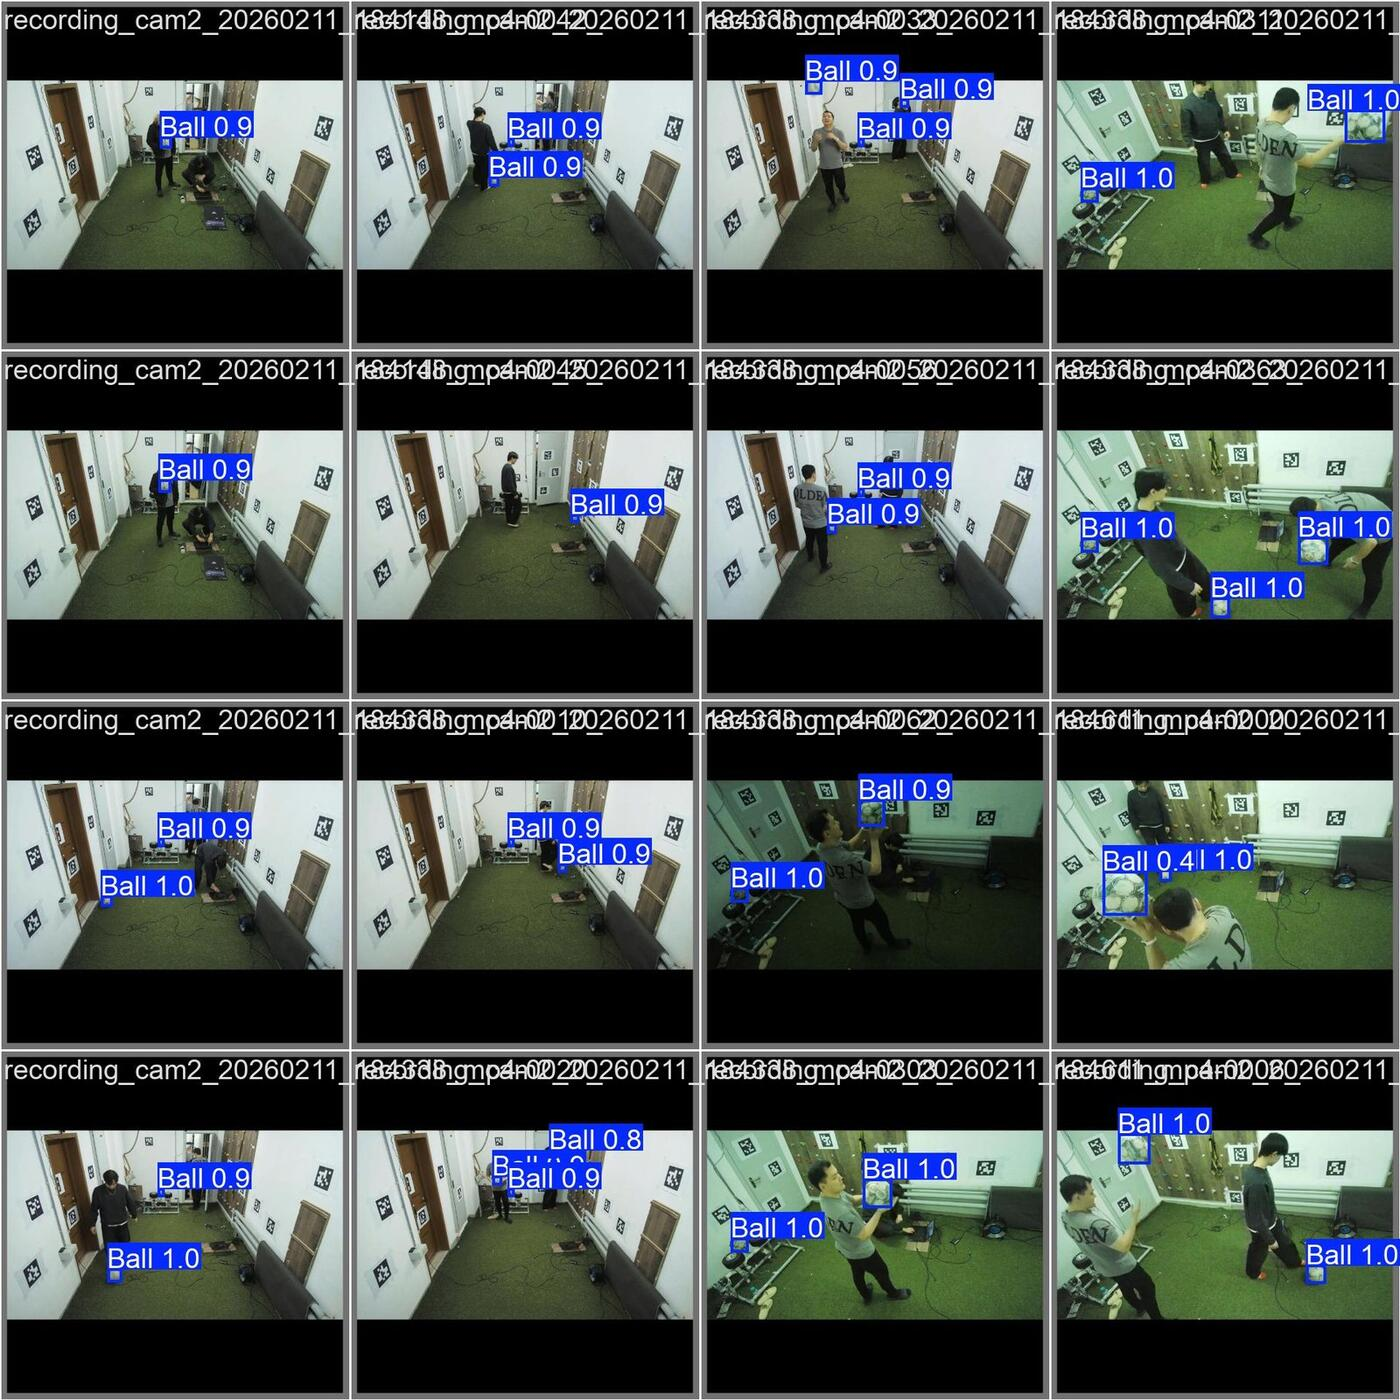
\includegraphics[width=0.9\textwidth]{figures/smoke_test_frame_1}
\caption{System architecture in action: live 4-camera arena view showing YOLO ball detection (green bounding box), MMPose skeleton overlay (COCO 17-keypoint), and 3D triangulated positions during continuous operation.}
\label{fig:3_3}
\end{figure}

\section{Intrinsic Calibration Pipeline}

\subsection{Board Specification and Detection}

A ChArUco board of 5 columns $\times$ 7 rows of squares (size of the square 21.5 cm) is used. ArUco markers embedded in alternate squares are used to provide identifier numbers for particular corners of the board that can be used for partial-board detection. The script streamlines the image collection process: the stream from all four cameras is used, the ChArUco corners are detected in each frame and the corner number is automatically saved when the number of detected corners is greater than 25, and the detection is stable for 3 seconds. This hands-free method ensures enough pose diversity without operator timing errors.

\subsection{Calibration Procedure}

Per-camera calibrating is done independently. For each camera, OpenCV \cite{ref27} is used to estimate intrinsic matrix $K$ and distortion coefficients ($k_1$, $k_2$, $p_1$, $p_2$, $k_3$) using minimisation of the reprojection error for all the collected frames. A good 30 valid frames per camera is aimed at. Frames with less than 25 corners detected are dropped before calibration.

The intrinsic calibration is done at 1280 $\times$ 720 resolution, which is the resolution that the system operates with. Calibrating at a different resolution than operation introduces a scaling error in the focal length and principal point, which would propagate as a systematic triangulation bias.

\subsection{Output and Validation}

Calibration outputs per-camera $K$ matrix and distortion vector, stored as JSON files in \path{garage_lab_combined/cal/intrinsics/}. Per-camera reprojection error is computed over the full calibration frame set as a quality indicator. Values in the range of 2--8 pixels are considered acceptable for this application.

\section{Extrinsic Calibration Pipeline}

\subsection{AprilTag Detection}

Twenty-four AprilTag markers (family tag36h11, IDs 0--23, 21.5 cm side length) are affixed to the arena walls at pre-measured world-frame positions stored in the calibration configuration. The script \texttt{calibrate\_extrinsics\_apriltag\_robust.py} runs AprilTag detection on still frames captured from each camera and assembles a set of PnP correspondences: for each detected tag corner, a 3D world position and a 2D image position.

\subsection{Robust PnP Optimisation}

Camera pose ($R$, $T$) is estimated for each camera via PnP with iterative refinement. An outlier rejection step with sigma-scale = 2.0 discards tag corner observations whose reprojection error exceeds two standard deviations of the residual distribution. This step eliminates the influence of misdetected tags or physical measurement errors in tag positions. The result is a per-camera rotation matrix $R$ and translation vector $T$ defining the camera's position and orientation in the world frame.

\subsection{Overlay Validation}

Extrinsic quality is validated visually by reprojecting the known AprilTag corner positions back into each camera image using the estimated ($K$, $R$, $T$) and overlaying the reprojected corners on the captured frame. When reprojected corners align tightly with detected corners across all cameras, the extrinsic calibration is considered valid. This validation is performed after any physical camera movement and before any data collection session.

\section{Multi-Camera Synchronisation}

The four Hikvision DS-E12 cameras have no hardware synchronisation signal. Software synchronisation is achieved through a flashlight sync marker protocol: a handheld flashlight is flashed briefly at the start of each recording session, creating a detectable brightness spike in all four camera streams simultaneously. Frame alignment is performed by finding the flashlight spike frame in each stream and offsetting the subsequent frames accordingly.

For the ground-truth evaluation sessions, which use static holds of 3--4 seconds, synchronisation accuracy of $\pm$ 2 frames (approximately 130 ms at 15 FPS) is acceptable, as the target is stationary during the hold window. For the dynamic validation clips, synchronisation accuracy would directly impact the quality of triangulation; larger temporal offset between cameras would make the apparent parallax of a moving ball larger which would introduce triangulation error.

A minimum of two cameras is required for triangulation, 3 or more cameras are targeted when experimental data collection is performed. The detection and triangulation code imposes a configurable limitation for the number of cameras needed (2 is used for the evaluation experiments), as well as stores the number of cameras used in each frame for post-hoc analysis.

\section{3D Triangulation}

\subsection{Ball Triangulation}

For each frame with a ball detection reported in two or more cameras with a confidence larger than the configured threshold value (0.25--0.45 and depends on each experiment) by the YOLO object detector, the 2D bounding box centre coordinates are combined into a set of ray equations using the ($K$, $R$, $T$) parameters collected per camera. The DLT method constructs a matrix $A$ which has the following property: a point $P$ in 3D will satisfy $A \cdot P = 0$ in a homogeneous least-squares sense. SVD of $A$ returns $P$ as the right singular vector corresponding to the smallest singular value \cite{ref1}.

\subsection{Pose Joint Triangulation}

For each of the COCO keypoints, the same procedure is followed using the 2D keypoint coordinate from each camera where the joint confidence exceeds the pose confidence threshold (0.35) and the joint is observed by at least 3 cameras. And the minimum number of cameras for pose triangulation is higher when compared to ball triangulation (3 versus 2) since joint observations are naturally more noisy when compared to ball centre estimates.

\subsection{Quality Filtering}

After the application of triangulation, two filters of quality are implemented:

\textbf{Reprojection error check:} The triangulated 3D point is projected into each contributing camera using the known ($K$, $R$, $T$) parameters. If the pixel distance between the projected position and the original detection is larger than the maximum reprojection error threshold (14--18 pixels depending on experiment), the point is discriminated as an outlier and removed from further processing of that frame.

\textbf{EMA smoothing:} Accepted 3D points are smoothed using an Exponential Moving Average filter with smoothing coefficient $\alpha = 0.25$. This suppresses frame-to-frame jitter while preserving the trajectory of a slowly moving target. The smoothed position is used as input to the ballistic solver.

\section{Ballistic Solver and Targeting Logic}

\subsection{Target Vector Computation}

The ballistic solver takes as input the current 3D world-frame target position $T = (T_x, T_y, T_z)$ in millimetres, sourced from the EMA-filtered and confidence-gated triangulated joint position. The BLM pivot point (launch origin) is a fixed, calibrated world-frame coordinate $B = (B_x, B_y, B_z) = (600, 1560, 500)$ mm.

The targeting vector from launcher to target is:

\begin{equation}
\Delta X = T_x - B_x \label{eq:3_1}
\end{equation}

\begin{equation}
\Delta Y = T_y - B_y \label{eq:3_2}
\end{equation}

\begin{equation}
\Delta Z = T_z - B_z \label{eq:3_3}
\end{equation}

The horizontal ground distance from launcher to target is:

\begin{equation}
D_{\text{horiz}} = \sqrt{\Delta X^2 + \Delta Y^2} \label{eq:3_4}
\end{equation}

\subsection{Yaw Angle Computation}

The required yaw (horizontal rotation) angle of the launcher to point at the target in the arena plane is:

\begin{equation}
\theta_{\text{yaw}} = \text{atan2}(\Delta Y, \Delta X) \label{eq:3_5}
\end{equation}

This is measured relative to the launcher's reference direction (pointing along the positive X axis). The result is converted to degrees and offset by the configured yaw trim parameter \texttt{-{}-yaw-trim-deg}, which compensates for any mechanical zero offset in the stepper motor homing procedure.

\subsection{Pitch Angle Computation}

The pitch angle is derived from the projectile motion equations (2.2)--(2.4). For a target at horizontal distance $D_{\text{horiz}}$ and height difference $\Delta Z$, the required pitch angle $\theta_{\text{pitch}}$ for a given initial ball speed $v_0$ satisfies:

\begin{equation}
\Delta Z = D_{\text{horiz}} \cdot \tan(\theta_{\text{pitch}}) - \frac{g \cdot D_{\text{horiz}}^2}{2 \cdot v_0^2 \cdot \cos^2(\theta_{\text{pitch}})} \label{eq:3_6}
\end{equation}

This is a transcendental equation in $\theta_{\text{pitch}}$. For applied launch distances in the arena (2000--5000 mm) and the chosen ball speeds, some numerical solving of the equation is done. To minimise flight time and to enhance targeting precision for a moving athlete, the lower-angle solution is chosen.

The result is compensated by the pitch trim parameter \texttt{-{}-pitch-trim-deg} to eliminate mechanical offset.

\subsection{Wheel RPM Computation}

Wheel RPM is proportional to desired initial ball speed $v_0$. The empirical mapping of the RPM and the ball speed is set up by calibration shots. A parameter \texttt{-{}-speed-scale} can be used to do runtime adjustment without changes to the firmware.

\subsection{Why This Is Non-Trivial}

The targeting computation is not a look-up table or pre-programmed direction. There are a couple of reasons that make it a very real-time control challenge. First, the target $T$ is changed every frame (at 15 FPS) when the athlete is moving, and the solver is required to run its calculation within a single frame time (approximately 67 ms) to not issue stale commands. Second, gravity serves to couple pitch angle to ball speed: the same target can be hit at multiple ($\theta$, $v_0$) combinations, and the solver is faced with having to choose the physically valid lower-angle solution and verify that it is in the mechanical range of the launcher stepper (nominally $\pm$ 30 degrees from horizontal). Third, the BLM stepper motor has a finite step resolution, so the solver rounds to the nearest achievable step position and logs the angular residual error for post-session analysis. Fourth, the BLM's mechanical zero (the position after \texttt{setzero}) must be registered to the world-frame coordinate system, and this registration is performed through the yaw and pitch trim calibration procedure validated in the aim-only tests (Section 5.6).

\subsection{Dynamic Target Tracking Behaviour}

The system operates as a state machine with three targeting states. In the \textbf{ACQUIRING} state, the joint has been detected in fewer than the minimum required cameras, or the EMA-filtered position has not yet stabilised, and no command is dispatched. In the \textbf{LOW\_CONFIDENCE} state, the detection confidence is below threshold, or the joint position has changed by more than 50 mm in the last 10 frames; the last valid command is held and the decision is logged as LOW\_CONFIDENCE. In the \textbf{READY} state, the joint position is stable (movement below 50 mm over 10 frames) and confidence is above threshold; the ballistic solve is executed and the serial command is dispatched.

A transition from READY back to ACQUIRING occurs if the joint disappears from the camera views (e.g., the athlete moves behind a wall or crouches below the camera field of view). The system does not fire in any other state than that of the E-STOP cleared (READY).

\section{Safety Architecture}

\subsection{E-STOP Latch}

An Emergency Stop function is designed as a software latch in the launcher runtime process. When a user types \texttt{estop} in the runtime terminal, all the motor commands are immediately stopped and the latch is placed. The system does not permit any additional actuation commands until \texttt{clear} is explicitly typed by the operator to release the latch. The measured response time from entry into the \texttt{estop} command to stop of the motor has a time of less than 100 ms.

\subsection{Multi-Level Gating}

Before any actuation command is dispatched, the following checks are performed in sequence. First, the \textbf{E-STOP check} verifies that the latch is cleared. Second, the \textbf{camera count check} confirms that at least two cameras have contributed to the current triangulation. Third, the \textbf{confidence check} ensures that detection confidence exceeds threshold for all contributing cameras. Fourth, the \textbf{zone check} verifies that the target coordinate falls within the defined safe operating zone (nominally the central arena area; coordinates near walls or outside the arena bounds are rejected as OUT\_OF\_RANGE). Fifth, the \textbf{stability check} confirms that the target is in READY state (see Section 3.8.6).

Failure at any check results in the decision being logged as the appropriate failure category and no command being sent.

\subsection{Six-Stage Integration Checklist}

Integration of the full system follows a mandatory staged protocol to prevent unsafe operation before each component has been validated in isolation. The six stages are as follows. \textbf{Preflight} verifies the camera stream, calibration files, and serial line. \textbf{ESP32 Only} tests all motor commands via direct serial terminal with no camera or BLM active. \textbf{Runtime Without Cameras} injects synthetic UDP target packets to verify solver and safety gating logic. \textbf{Live Aim-Only} runs the full pipeline active, with motors commanded to correct aim angles and no ball loaded. \textbf{Safety Verification} performs E-STOP, latch, link-loss, and zone-rejection tests under live conditions. \textbf{Controlled Firing} conducts single shots with ball loaded, one at a time, with the operator present.

Each stage has defined pass criteria. A stage is not passed until all criteria are met and evidence (terminal logs, video, JSONL records) is archived. Stage 6 defines full cycle reliability testing.
